\chapter{Computational Methods with Sparse Matrices}
\label{chap:sparseMatrix}
{
	\hypersetup{linkcolor=black}
	\minitoc
}
\clearpage 



\underline{\textbf{Computational Methods with Sparse Matrices}}

\section{Introduction}

To better understand the advanced ODE solvers and their connection with
computational linear algebra, we first need to briefly consider the solution
methods underlying stiff systems of ODEs and their corresponding matrix algebra.
In general some classes of multistep methods are used for the solution of a
system of ODEs of size $N \times N$ of the form:
\begin{equation}\label{E:linde}
    \bm{y'}= \frac{d{\bm{y}}}{dt} = {\bm {f}}\ts (t,{\bm{y}}), \quad {\bm{y}}(t_0)= {\bm {a}}
\end{equation}

To advance the solution at time $t$ from one mesh point to the next, considering
a discrete time mesh $\{t_0,t_1,t_2, ...,t_n\}$, multistep methods make use of
several past values of the variable $y$ and its rate of change $f$ with respect
to time $t$. The general form of a \mbox{$k$-step} multistep method is:
\begin{equation}\label{E:linde}
    \sum_{i=0}^k \alpha_i y_{j+i} = h \sum_{i=0}^k \beta_i f_{j+i},
\end{equation}
where $\alpha_k=1$, $\alpha_i$  and $\beta_i$  are constants and depend on the
order of the method, $h$ is the stepsize in time and $j$ denotes the mesh
number. The well-known family of Adams methods:
\begin{equation}\label{E:linde}
    y_{j+k} = y_{j+k-1} + h \sum_{i=0}^{k} \beta_i f_{j+i},
\end{equation}
which use mostly the past values of $f$, are the best-known multistep methods for
solving nonstiff problems. Each step requires the solution of a nonlinear system
and often a simple functional iteration with an initial guess, or a predictor
estimate, is used to advance the integration which is terminated by a
convergence test. For stiff problems, where sudden changes in the variables can
occur (i.e. where there are sharp changes in variables $y$ over small time
intervals say) simple iteration methods lead to an unacceptable restriction of
the stepsize and functional iteration fails to converge. Thus, stiffness forces
the use of implicit methods, with infinite regions of stability, when there is
no restriction on the choice of the stepsize $h$. The backward difference
formulae (BDF) methods with unbounded region of absolute stability were the
first numerical methods developed for solving stiff ODEs (Curtiss and
Hirschfelder, 1952). The BDF methods used in ODE solvers, are of the general
form:
\begin{equation}\label{E:linde}
    \sum_{i=0}^k \alpha_i y_{j+i}= h \beta_k f_{j+k}
\end{equation}
where $\alpha_i$  and $\beta_k$ are coefficients of $k^{th}$ order,
$k \rm -step$ BDF methods.  As noted earlier, a simple functional iteration will
usually fail to converge when problems are stiff and instead some form of Newton
iteration is used for the solution of the resulting nonlinear system. The Newton
iteration involves the solution of an $N \times N$ matrix $P$,
\begin{equation}\label{E:linde}
    P \approx I + h \beta_k J
\end{equation}

where $J = \frac{\partial{f}}{\partial{y}}$ is the associated Jacobian matrix
and $I$ is an $N \times N$ identity matrix.

\newpage
The solution to this linear algebraic system contributes significantly to the
total computational time for the stiff problems, as well as affecting the
accuracy of the solution ( and hence, also affecting computational time).  For
stiff problems the ODE solvers use a modified Newton iteration that allows time
saving strategies for the computation, storage and the use of the Jacobian
matrix.  When solving a linear algebraic system there are generally two classes
of solution methods, direct methods and indirect methods.  The most common
direct method used to solve linear systems is the Gaussian Elimination method
based on factorization of the matrix in lower and upper triangular factors. The
GEAR, LSODE and VODE solvers all use such a method for the solution of the
resulting linear system.  The simplest iterative scheme used to solve linear
systems is the Jacobi iteration, although the more sophisticated solution
methods of Krylov subspace methods, based on a sequence of orthogonal vectors
and matrix-vector multiplications, have been widely used in practical
applications such as computational fluid dynamics.  The ODE solvers, LSODPK and
VODEPK implement preconditioned Krylov iterative techniques for the solution of
the resulting linear system.

\section{Sparse Matrices}

Definitions: A sparse matrix is a matrix with a large number of zero elements,
compared to the total number of elements. Alternatively, we say a matrix can be
considered as sparse if the number of nonzero elements $nnz \ll (N^{2} + N)/2$.

The Newton iteration solution technique introduces a large amount of
computational overhead necessary to solve the linear algebraic system related to
the Jacobian matrix of a stiff system of ODEs. Some matrices have particular
structure that are more convenient for computational purposes, for example upper
triangular matrices, lower triangular matrices and banded matrices.  Ordering
the columns of a matrix can often make its lower and upper (LU) factors sparser.
The simplest such ordering is to sort of columns or rows by nonzero count (i.e
by the nonzero elements).  This is often a good ordering scheme for matrices
with very irregular structure, especially if there is a great variation in the
nonzero counts of rows or columns. Therefore, although by ordering of matrices
the position of nonzero elements will be different and the resulting ordered
matrix will have a completely different structure, this will not change the
physical problem in any way and the reordering will have a significant impact on
the solution techniques. As an example, if Gaussian Elimination method is used
(e.g. in the GEAR, LSODE and VODE solvers) on an ordered matrix, then none or
very few fill-ins (of originally zero entries) will occur in the factorization
processes, i.e. the L and U parts of the LU factorization will have the same
structures as the lower and upper parts of the original matrix, respectively.
Thus, ordering allows the sparsity structure of the system to be preserved in
the factorization processes.

\newpage
\section{Matrix Sparsity and Graph Theory}

A graph $G = \{v,E\}$ consists of a set of vertices $v\text{(nodes)}$ and a
set of edges $E$ connecting the vertices.  A graph can be used to represent the
nonzero pattern of a sparse matrix.  Any symmetric sparse matrix can be
represented by a graph $G$ where there is an edge from vertex
$i\ts\text{(row)}$ to vertex $j\ts\text{(column)}$ and a letter or symbol
represents the nonzero entry, e.g. $a_{ij}$:

Associated with each graph is an adjacency matrix $A = (a_{ij})$:

\begin{equation*}
    (a_{ij})=\begin{cases}
        1, & \text{if an edge exists},\\
        0, & \text{otherwise}.
    \end{cases}
\end{equation*}

The degree of a node in a graph is the number of nodes adjacent to it (or the
number of edges connected to it).
\noindent
\vskip 10pt
\noindent
{\bf\underline {Example 1}}
\vskip 10pt
\noindent
Consider the following matrix $A$ and its corresponding adjacency graph.
\begin{table}[H]
  \begin{minipage}[b]{0.50\linewidth}\centering
    \vskip 10pt
    $A=
    \begin{bmatrix}
      1 & 1 & 0 & 0 & 1 \\
      1 & 1 & 1 & 1 & 0 \\
      0 & 1 & 1 & 1 & 0 \\
      0 & 1 & 1 & 1 & 1 \\
      1 & 0 & 0 & 1 & 1
    \end{bmatrix}$
    \vspace{5mm}
  \end{minipage}
  \begin{minipage}[b]{0.49\linewidth}
    \includegraphics[width=7cm]{main/07/extex_1.tikz}
  \end{minipage}
\end{table}
\vskip7mm
\noindent
The following MATLAB .m file produces the adjacency graph of matrix A:

\noindent
{\small
\begin{lstlisting}
%Example 1 - Adjacency graph using gplot function
A=[1 1 0 0 1;1 1 1 1 0;0 1 1 1 0;0 1 1 1 1;1 0 0 1 1];
% Enter the Cartesian coordinates for the vertices
xy=[1 1; 2 2; 5 2; 4 1; 3 1];
gplot(A,xy,'k-*');% marking the elements using * in black font
axis([0 6 0 3]);
text(1,0.9,'1');
text(2,2.1,'2');
text(5,2.1,'3');
text(4,0.9,'4');
text(3,0.9,'5');		
\end{lstlisting}}

\newpage
{\bf\underline {Example 2}}

\noindent
Consider the following matrix $A$ and its corresponding adjacency graph.
\begin{table}[H]
  \begin{minipage}[b]{0.50\linewidth}\centering
    \vskip -10pt
    $A=
    \begin{bmatrix}
      1 & 1 & 0 & 0 & 1 & 0\\
      1 & 1 & 1 & 0 & 0 & 1\\
      0 & 1 & 1 & 0 & 0 & 0\\
      0 & 0 & 0 & 1 & 1 & 0\\
      1 & 0 & 0 & 1 & 1 & 1\\
      0 & 1 & 0 & 0 & 1 & 1\\
    \end{bmatrix}$
    \vspace{3mm}
  \end{minipage}
  \begin{minipage}[b]{0.49\linewidth}\
    \includegraphics[width=7cm]{main/07/extex_2.tikz}
  \end{minipage}
\end{table}
\vskip -15pt
\noindent
\ttfamily
\begin{lstlisting}
%Example 2 - Adjacency plot
A=[1 1 0 0 1 0;1 1 1 0 0 1;0 1 1 0 0 0;0 0 0 1 1 0;
    1 0 0 1 1 1; 0 1 0 0 1 1];
xy=[2 1;3 1;4 1;1 2;2 2;3 2];
gplot(A,xy,'k-*');
axis([0 5 0 3]);
text(2,0.9,'1');
text(3,0.9,'2');
text(4,0.9,'3');
text(1,2.1,'4');
text(2,2.1,'5');
text(3,2.1,'6');
%End											
\end{lstlisting}

\rmfamily
\noindent
In MATLAB the function $\emph{spy}$ plots the sparsity pattern (i.e. the
non-zero elements) of any matrix A.
\vskip 10pt
\noindent
{\bf\underline {Example 3}}
\vskip 3pt
\begin{table}[H]
  \begin{minipage}[b]{0.50\linewidth}
    \noindent
    Enter the matrix A in MATLAB
    \noindent
    \begin{lstlisting}
>> A=[1 0 2 3 0
      0 0 0 5 0
      0 1 0 0 8
      1 0 0 0 4
      0 0 6 7 0]

Followed by the command spy
>> spy(A)
    \end{lstlisting}
    \vspace{5mm}
    \rmfamily
    \noindent
    MATLAB will produce the sparsity pattern \hfill\break
    \noindent
    (nonzero elements) for matrix $A$ as:
    \vspace{10mm}
  \end{minipage}
  \begin{minipage}[b]{0.49\linewidth}
    %\includegraphics{extex_3.tikz}
      \begin{tikzpicture}
    \begin{axis}
        [   unit vector ratio* = 1 1 1
        ,   y dir = reverse
        ,   xmin = 0
        ,   ymin = 0
        ,   xmax = 6
        ,   ymax = 6
        ,   xlabel = {nnz=10}
        ,   width = \linewidth
        ,   xtick = {1,2,3,4,5}
        ,   ytick = {1,2,3,4,5}
        ,   title = {Fig 3. Sparsity pattern for matrix $A$}
        ]
        \addplot[only marks] coordinates
        {   (1,1) (1,4) (2,3) (3,1) (3,5) (4,1) (4,2) (4,5) (5,3) (5,4)
        };
    \end{axis}
\end{tikzpicture}

  \end{minipage}
\end{table}
\noindent
\vskip -20pt
The number of nonzero elements in matrix $A$ is $10$ and this is noted by
$nnz=10$ in Fig. 3.

\newpage
\noindent
{\bf\underline {Example 4}}
\vskip 3pt
Define the matrix $A$, from Example 2, in MATLAB, followed by the command
spy(A), gives:

%\begin{table}[H]
  \begin{minipage}[  ]{0.50\linewidth}
  %  \vskip 5pt
    \begin{lstlisting}
>> A=[1 1 0 0 1 0
      1 1 1 0 0 1
      0 1 1 0 0 0
      0 0 0 1 1 0
      1 0 0 1 1 1
      0 1 0 0 1 1]

>> spy(A)
    \end{lstlisting}
  %\vspace{25mm}
  \end{minipage}
  \begin{minipage}[]{0.49\linewidth}
    %\begin{center}
    %  \includegraphics[width=7cm]{main/07/Example4.tikz}
    %\end{center}
    \centering
	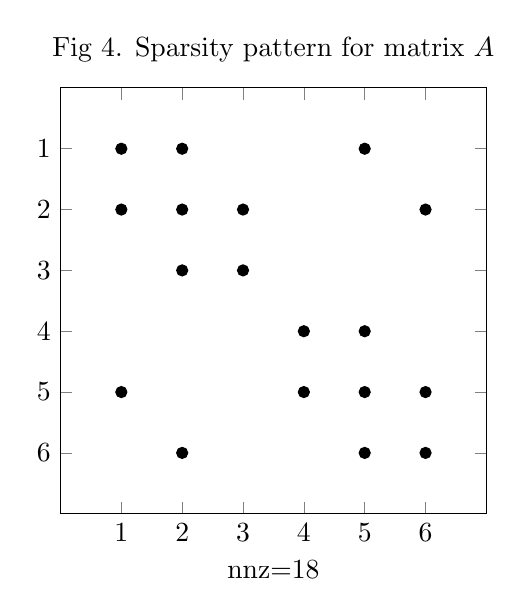
\begin{tikzpicture}
    \begin{axis}
        [   unit vector ratio* = 1 1 1
        ,   title = {Fig 4. Sparsity pattern for matrix $A$}
        ,   y dir = reverse
        ,   xmin = 0
        ,   ymin = 0
        ,   xmax = 7
        ,   ymax = 7
        ,   xlabel = {nnz=18}
        ,   xtick = {1,2,3,4,5,6}
        ,   ytick = {1,2,3,4,5,6}
        ,   scale = 0.95
        ]
        \addplot[only marks] coordinates
        {   (1,1)(1,2)(1,5)
            (2,1)(2,2)(2,3)(2,6)
            (3,2)(3,3)
            (4,4)(4,5)
            (5,1)(5,4)(5,5)(5,6)
            (6,2)(6,5)(6,6)
        };
    \end{axis}
\end{tikzpicture}

  \end{minipage}
%\end{table}

%\vskip -10pt
%\noindent
%{\bf\underline {3. Sparse Matrices Storage and Reordering}}
%\vskip 5pt
%\noindent
%{\bf\underline {3.1 Storing Sparse Matrices}}
%\vskip 3pt

\section{Sparse Matrices Storage and Reordering}
\subsection{Storing Sparse Matrices}
The coordinate scheme is the most preferred way to specify a sparse matrix in
the form of an unordered set of triples $(i,j, a_{ij})$. Consider the following
example.
\vskip 3pt
\noindent
{\bf\underline {Example 5}}
\vskip 3pt
\noindent
Consider a $5\times5$ sparse matrix A:
\vskip 3pt
\noindent
$
A=
\begin{bmatrix}
1 & 0 & 2 & 3 & 0 \\
0 & 0 & 0 & 5 & 0 \\
0 & 1 & 0 & 0 & 8 \\
1 & 0 & 0 & 0 & 4 \\
0 & 0 & 6 & 7 & 0
\end{bmatrix}
$
\noindent
\vskip 1pt
\noindent
\vskip 1pt
\noindent
where $i$ denotes the row and $j$ denotes the column numbers. Note that the
number of nonzero elements is 10. The coordinate scheme representation of matrix
$A$ is shown in the following table:
\vskip 1pt
\noindent
\begin{center}
    \begin{tabular}{ r | c c c c c c c c c c }
    Subscripts  & 1 & 2 & 3 & 4 & 5 & 6 & 7 & 8 & 9 & 10 \\
    \hline
    $i$         & 1 & 4 & 3 & 1 & 5 & 1 & 2 & 5 & 3 & 4 \\
    $j$         & 1 & 1 & 2 & 3 & 3 & 4 & 4 & 4 & 5 & 5 \\
    $a_{ij}$    & 1 & 1 & 1 & 2 & 6 & 3 & 5 & 7 & 8 & 4 \\
\end{tabular}
\end{center}
\vskip 4pt
\noindent
From the table, the second column $i = 4$, $j= 1$. This means the matrix element
is 1 in this example.  For sparse matrices, MATLAB uses the same approach to
store the nonzero elements and their indices. The $\emph{sparse}$ function
generates matrices in the MATLAB sparse storage organisation. It converts a full
matrix to sparse form by only considering the nonzero elements.

\newpage
\noindent
{\bf\underline {Example 6}}
\vskip 10pt
\noindent
Consider matrix $A$ in Example 5, with 10 nonzero elements. To convert matrix
$A$ to sparse form in MATLAB use $\emph{sparse}$ function:
\noindent
{\ttfamily
\begin{lstlisting}
>> A=[
1 0 2 3 0
0 0 0 5 0
0 1 0 0 8
1 0 0 0 4
0 0 6 7 0];

>> sparse (A)
ans =
   (1,1)        1
   (4,1)        1
   (3,2)        1
   (1,3)        2
   (5,3)        6
   (1,4)        3
   (2,4)        5
   (5,4)        7
   (3,5)        8
   (4,5)        4
\end{lstlisting}
}
%\vskip 5pt
%\noindent
%{\bf\underline {3.2 Matrix Storage Information}}
\subsection{Matrix Storage Information}
%\vskip 10pt
%\noindent
A matrix can be stored in full or only by its nonzero elements. For example, it
will have the same entries and their elements, eigenvalues and determinants are
equal but the computation storages are different.  In general, the computation
storage of sparse matrices is proportional to the number of nonzero elements.
The $\emph{whos}$ command in MATLAB provides the general information about
matrix size and storage as shown in Example 5.
\vskip 10pt
\noindent
\begin{center}
    \begin{tabular}{ l l l }
        \hline
        Name      & Size     & Bytes Class  \\
        \hline
        Full A    &$5\times5$& 200 double\\
        Sparse A  &$5\times5$& 144 double\\
    \end{tabular}
\end{center}
\vskip 10pt
\noindent
The number of bytes used in the sparse version is less than the full version,
since the zero elements are not stored.  For a large scale sparse matrix system,
this leads to significant savings in data storage.  For example for a
$1100\times 1100$ matrix the storage saving is significant:-
\vskip 1pt
\noindent
\ttfamily
\begin{lstlisting}
full      1100x1100          9680000	double
sparse    1100x1100          5004	    double
\end{lstlisting}
\rmfamily
%\vskip 2pt
\noindent
For full matrices, MATLAB stores every matrix element internally.   Zero-valued
elements require the same amount of storage space as any other matrix element.
For large matrices with a high percentage of zero-valued elements, this scheme
significantly reduces the amount of memory required for data storage.

\newpage
\section{Reordering and Matrix Bandwidth}
%\noindent
%{\bf\underline {4. Reordering and Matrix Bandwidth}}
%\vskip 10pt
%\noindent
During the process of matrix factorization into a product by methods such as
Gaussian elimination and Cholesky factorization, there will always be a problem
with fill-in that is generating additional nonzero elements during the
elimination process (i.e. row operation).   Hence we are unable to take
advantage of the sparsity feature of the original matrix and end up wasting both
storage and computational time.  Therefore the problem is how to perform row
operations whilst minimizing the fill-in of nonzero elements.  One way to
achieve this is to try to position the nonzero elements near the main or
principal diagonal, so that reordering of rows and columns will not result in
additional nonzero elements.  The process of moving the nonzero element near the
principal diagonal is the same as reducing the profile or the bandwidth of the
matrix.

\vskip 5pt
\noindent
Consider an $n \times n$ matrix $A=(a_{ij})$.  If all matrix elements are zero
outside a diagonally confined band whose range is determined by constants $p$
and $q$;

\vskip 7pt
\noindent
\phantom{.} \hskip 20mm $a_{ij}=0$   $\text{if}$   $j<i-p$   $\text{or}$ $j>i+q$; $p,q \geq 0$
\vskip 7pt
\noindent
(or $j-i>p$, or $i-j>q$; $p, q \geq 0$ ), where $p$ and $q$ are the distances
above and below the main diagonal, then the bandwidth  $bw$ is given by
$bw=p+q+1$ (in other words, it is the smallest number of adjacent diagonals to
which the non-zero elements are confined).
\vskip 6pt
\noindent
A matrix is called a band matrix or banded matrix if its bandwidth is reasonably
small.
\vskip 6pt
\noindent
A band matrix with $p=q=0$ is a diagonal matrix; $
A=
\begin{bmatrix}
1 & 0 & 0 & 0  \\
0 & 1 & 0 & 0  \\
0 & 0 & 1 & 0  \\
0 & 0 & 0 & 1
\end{bmatrix}
$
\vskip 8pt
\noindent
A band matrix with $p=q=1$ is a tridiagonal matrix; $
B=
\begin{bmatrix}
1 & 1 & 0 & 0  \\
1 & 1 & 1 & 0  \\
0 & 1 & 1 & 1  \\
0 & 0 & 1 & 1
\end{bmatrix}
$
\vskip 8pt
\noindent
The indices of the nonzero elements for matrix $B$ are given in the following
table, using the conventional numbering used in MATLAB.
\vskip 10pt
\begin{center}
    \begin{tabular}{ c  c  c }
    $i$   &$j$   &$[i,j]$\\
    \hline
     1    & 1    & [1,1] \\
     2    & 1    & [2,1] \\
     1    & 2    & [1,2] \\
     2    & 2    & [2,2] \\
     3    & 2    & [3,2] \\
     2    & 3    & [2,3] \\
     3    & 3    & [3,3] \\
     4    & 3    & [4,3] \\
     3    & 4    & [3,4] \\
     4    & 4    & [4,4] \\
    \end{tabular}
\end{center}
\noindent
\vskip 5pt
\noindent
Therefore, the difference between i and j for each nonzero entry is either 0 or
1; hence the maximum distance is 1, i.e. in MATLAB the bandwidth calculation for
a tridiagonal matrix $T$ is performed by the following commands:-
\vskip 2pt
\noindent
\begin{lstlisting}
% Calculate bandwidth of a given matrix

>> T =[
     1     1     0     0
     1     1     1     0
     0     1     1     1
     0     0     1     1]

>> [i,j]=find(T);
>> bw=max(i-j)

bw =
     1
\end{lstlisting}
\vskip 12pt
\noindent
Note:
\vskip 4pt
\noindent

\begin{lstlisting}
[i,j]=find(T); %returns the row and column indices for
               % the nonzero entries
bw=max(i-j)    %returns an array the same size as i
               %and j with the largest elements taken
               %from i or j.
               %the dimensions of i and j must match.
\end{lstlisting}
\vskip 2pt
\noindent
Note - in some textbooks and articles the bandwidth is given as $bw=p+q+1$ - the
bandwidth of a tridiagonal matrix is given as 3 (i.e. $1(L) + 1(U) + 1(D)$). 
Also, when $p=q=2$ one has a pentadiagonal matrix and so on. Also, an upper
triangular matrix is obtained when $q=0$, $q=n-1$, and similarly, with $p=n-1$,
$q=0$, a lower triangular matrix is obtained.
%\vskip 2pt
%\noindent
\newpage
%{\bf\underline {4.1 Cuthill and McKee Reordering}}
%\vskip 10pt
%\noindent
\subsection{Cuthill and McKee Reordering}
The most simple and popular method of minimizing the bandwidth was developed by
Cuthill and McKee (1969).  Later the method was improved by Alan George who
developed the Reverse Cuthill and McKee (RCM) method which is much more
effective than the original CM algorithm.  There are several other efficient
bandwidth reduction methods used in re-ordering of sparse matrices, namely
Minimum Degree Reordering method.
\vskip 12pt
\noindent
The Cuthill and McKee algorithm is outlined in the following steps:-
\vskip 12pt
\noindent
\begin{enumerate}
   \item For a given sparse symmetric matrix, plot the adjacency graph
       (alternatively if you have been given the adjacency graph, then it is
       useful to write down the corresponding adjacency matrix).
\vskip 2pt
   \item Look at all the nodes, and produce a table listing the node numbers and
       the number of connections (or degree).
\vskip 2pt
   \item Select the node with the lowest degree (say $n_1$) and write it down
       under a column heading `Result/Head'.  If there is more than one node
       with the same number of degree, then choose one of them and write it down.
\vskip 2pt
   \item Look at the nodes connected directly to node $n_1$, write down in the
       next column `Queue' the nodes that are connected to $n_1$, in the order
       with lowest degree (e.g. $n_2$, $n_3$, $n_4$) that has not appeared in
       the Result column before.
\vskip 2pt
   \item Extract the first node in the queue - say $n_2$, if $n_2$ has not been
       previously inserted in `Result' then write $n_2$ below $n_1$ and check
       again for the connections.  Since $n_4$ is already in the queue, you need
       to see if $n_2$ is connected to any other nodes, say $n_5$ write down in
       the queue column $n_4$ if $n_2$ was not connected to a new node, just
       leave a blank in the queue column.
\vskip 2pt
   \item Now, write down $n_3$ below $n_2$ in the Results column, and repeat
       step 4.
\vskip 2pt
   \item Repeat steps 4 to 6 until there are no more nodes left to be
       considered.
\vskip 2pt
   \item Look at your list in the column Result - and renumber these as new node
       numbers.
\vskip 2pt
   \item Continue until the size of the array Result is $n$ for an $n\times n$
       matrix (i.e. all nodes are included in the array).
 \end{enumerate}
\vskip 6pt
\noindent
Note:- If the selected node in column Results is not connected to any other
node, then we put a `-' in the corresponding position in the queue column.

\newpage
\vskip 8pt
\noindent
{\bf\underline {Example 7.1}}
\vskip 7pt
\noindent
Consider the following sparse matrix and its corresponding adjacency plot:
\vskip 2pt
\noindent
\begin{table}[H]
  \begin{minipage}[b]{0.50\linewidth}
    \vskip 5pt
    \begin{center}
      $A=
      \begin{bmatrix}
        1 & 0 & 0 & 0 & 1 & 0 & 0 & 0 \\
        0 & 1 & 1 & 0 & 0 & 1 & 0 & 1 \\
        0 & 1 & 1 & 0 & 1 & 0 & 0 & 0 \\
        0 & 0 & 0 & 1 & 0 & 0 & 1 & 0 \\
        1 & 0 & 1 & 0 & 1 & 0 & 0 & 0 \\
        0 & 1 & 0 & 0 & 0 & 1 & 0 & 1 \\
        0 & 0 & 0 & 1 & 0 & 0 & 1 & 0 \\
        0 & 1 & 0 & 0 & 0 & 1 & 0 & 1
      \end{bmatrix}$
    \end{center}
    \vspace{10mm}
  \end{minipage}
  \begin{minipage}[b]{0.49\linewidth}
    \begin{center}
      \includegraphics[width=5cm]{main/07/Fig7a.tikz}
    \end{center}
  \end{minipage}
\end{table}

